\documentclass{article}
\usepackage[utf8]{inputenc}
\usepackage[english]{babel}
\usepackage{graphicx}
\usepackage{cite}
\usepackage{url}
\usepackage{hyperref}
\usepackage{amsmath}
\usepackage{amssymb}
\usepackage{caption}
\usepackage{parskip}
\captionsetup{font=small, labelfont=bf, skip=2pt}
\setlength{\abovecaptionskip}{2pt}
\setlength{\belowcaptionskip}{4pt}

\title{ContVAR: Contrastive Graph Representation Learning for Protein Variant Function Prediction}
\author{}
\date{}

\begin{document}
\maketitle

\begin{abstract}
Determining the functional consequences of single amino acid variants (SAVs) remains a central challenge in computational biology. Existing variant effect predictors often optimize pathogenicity discrimination, whereas many downstream analyses require mutation-aware representations that preserve finer functional relationships and translate directly into Gene Ontology (GO)-level loss- and gain-of-function statements. We present ContVAR, a two-stage graph metric-learning and decoding pipeline. The first stage trains a mutation-aware encoder on residue graphs built from monomer structures, where node features concatenate amino-acid one-hot identities with per-residue ESM-2 embeddings; each residue graph uses a fixed-budget hybrid connectivity---$k$ sequence-index neighbors, $k$ $\mathrm{C}_\alpha$ spatial nearest neighbors, and $k$ stochastic long-range links (Gumbel top-$k$ sampling with inverse-cube distance weighting)---with edge attributes combining radial-basis-encoded distances, neighbor-type indicators, and normalized sequence separation, so message passing captures local packing and sparse non-local coupling without dense all-pairs edges. The encoder backbone is a residual two-layer GATv2 stack with edge-aware message passing. Encoder training proceeds in two phases: phase~0 GO semantic triplet pretraining across Molecular Function (MF), Biological Process (BP), and Cellular Component (CC), followed by phase~1 DMS contrastive specialization with a joint objective that averages (i) a global graph-level triplet loss with per-batch streaming semi-hard negative mining and (ii) a local mutation-site contrastive loss. The second stage trains three per-ontology feed-forward GO decoders (\texttt{FFNDecoder}) on top of frozen encoder embeddings with multi-label binary cross-entropy and class-balanced positive weights, including a dedicated \texttt{NULL\_FUNCTION} class for complete loss-of-function variants. Wild-type vs. variant decoder scores are then combined into per-GO LOSS/GAIN/NEUTRAL calls and a scalar \texttt{ContVAR\_fitness}. The pipeline logs encoder-side alignment, uniformity, MRR, and split-aware losses, and decoder-side mAP, macro F1, precision, recall, accuracy, and MCC under UniRef50 cluster-aware splits, supporting reproducible protein-family-level validation.
\end{abstract}

\section{Introduction}
The functional annotation of proteins and the accurate interpretation of single amino acid variants (SAVs) are essential for unraveling disease mechanisms, understanding oncogenic transformations, and guiding targeted therapeutics. Advances in high-throughput sequencing have produced large catalogs of coding variation; however, experimental characterization remains costly, leaving many variants classified as variants of uncertain significance (VUS).

Computational variant effect prediction (VEP) methods are therefore widely used. Classical approaches, such as SIFT~\cite{ng2001predicting}, PolyPhen-2~\cite{adzhubei2010method}, and CADD~\cite{kircher2014general}, rely on conservation and hand-crafted descriptors to estimate deleteriousness. More recent sequence-first models, including language-model-based paradigms~\cite{meier2021language,lin2023evolutionary}, improve zero/few-shot generalization by learning distributional constraints from large corpora. However, most VEP pipelines still optimize scalar pathogenicity signals rather than structured function-level objectives.

In parallel, automated protein function prediction has moved from sequence-similarity transfer to deep neural annotation models such as DeepGOPlus~\cite{kulmanov2019deepgoplus}, DeepFRI~\cite{gligorijevic2021structure}, TALE~\cite{cao2021tale}, and network-aware graph models such as DeepGraphGO~\cite{zhang2021deepgraphgo}. These methods are effective for wild-type GO assignment, but they are generally not designed around anchor--positive--negative mutation triplets, and thus do not directly enforce mutation-sensitive metric geometry.

\paragraph{Problem statement.}
Current literature leaves a practical gap between (i) ontology-aware representation learning and (ii) mutation-specific discrimination at protein-family split level. In our setting, this gap appears as follows: GO similarity supervision exists only as semantic pairs/triplets on cached protein graphs, while DMS training requires dynamic hard-negative selection over many candidate variants per family. A model that ignores either side tends to underperform for one of two goals---semantic organization (GO) or mutation separation (DMS). We therefore target a joint training regime that preserves GO-informed structure in initialization and then sharpens mutation-aware separation with explicit local supervision at the altered residue.

This work introduces ContVAR, a graph metric-learning framework that explicitly connects GO-structured semantic priors with DMS-driven contrastive supervision. ContVAR builds residue graphs from monomer coordinates (e.g., AlphaFold-predicted structures~\cite{jumper2021highly}), combines ESM-2 embeddings with residue identity encodings, and trains a shared encoder with ontology-specific phase~0 heads followed by phase~1 DMS specialization under a joint global+local objective.

\section{Related Work}

\subsection{Background concepts}
Metric learning on biological objects often uses triplet-style objectives to impose relative distances under weak labels. In protein representation learning, this strategy is attractive when categorical labels are incomplete but pairwise or ranking signals are available (e.g., mutational fitness ordering, semantic similarity). Graph neural networks additionally permit explicit spatial topology and residue-level context, which are difficult to capture with sequence-only encoders.

\subsection{Recent approaches}

\paragraph{Variant effect prediction.}
Early VEP tools rely on evolutionary conservation and biophysical heuristics. SIFT~\cite{ng2001predicting} classifies substitutions as tolerated or damaging by comparing amino acid properties at conserved positions derived from homologous sequences. PolyPhen-2~\cite{adzhubei2010method} combines sequence-based features with structural information (solvent accessibility, dihedral angles) in a Naïve Bayes classifier. CADD~\cite{kircher2014general} moves beyond single-residue heuristics by integrating dozens of heterogeneous annotations (conservation, regulatory context, protein features) into a single pathogenicity score via a trained support vector machine.

The advent of large protein language models opened a sequence-first paradigm for VEP. ESM-1v~\cite{meier2021language} performs zero-shot prediction of the effect of missense mutations by scoring sequences with a masked-language-model objective, demonstrating that evolutionary co-variation implicit in pre-training data captures functional constraints without explicit labels. ESM-2~\cite{lin2023evolutionary} scales this to 650M--15B parameters and achieves strong performance across multiple DMS benchmarks.

\paragraph{Protein function prediction.}
DeepGOPlus~\cite{kulmanov2019deepgoplus} combines per-residue CNN features over sequences with a sequence-similarity transfer step, reporting mAP gains over sequence-similarity alone across all three GO aspects. TALE~\cite{cao2021tale} uses a Transformer with a joint sequence-label embedding that ties GO term representation to sequence features, improving annotation on sparsely annotated functions. DeepFRI~\cite{gligorijevic2021structure} constructs residue contact graphs from PDB structures and applies graph convolutional networks, showing that structure-derived topology captures functional relationships missed by sequence alone. DeepGraphGO~\cite{zhang2021deepgraphgo} aggregates protein-protein interaction (PPI) networks with sequence features through a GNN, demonstrating large-scale multispecies GO prediction.

Despite this progress, the two families address adjacent but not identical problems: VEP models output variant-level disruption scores, while GO annotation models assign terms to wild-type sequences. Neither family explicitly enforces mutation-sensitive metric geometry that respects GO-level functional differences.

\subsection{Comparative discussion}
Compared with pure sequence models, structure-aware encoders can represent non-local residue couplings and interface geometry. Compared with direct GO classifiers, metric objectives are more flexible for ranking and retrieval-style analyses. ContVAR combines these two aspects by first injecting GO semantics in latent geometry (phase~0), then refining mutation separation in phase~1 with DMS triplets and local residue-level contrastive supervision.

\subsection{Research gap}
The missing component in many prior pipelines is a \emph{single training flow} that (a) starts from GO-semantic constraints, (b) operates on mutation-level triplets, and (c) explicitly supervises both whole-graph and mutation-site representations under memory-aware hard-negative mining. This gap motivates the ContVAR design.

\section{Methodology}

\subsection{Overall Framework}
Figure~\ref{fig:pipeline} summarizes the full workflow from structure-derived residue graphs through encoder training (phases~0--1) to GO decoding and variant function-change inference.

\begin{figure}[!t]
  \centering
  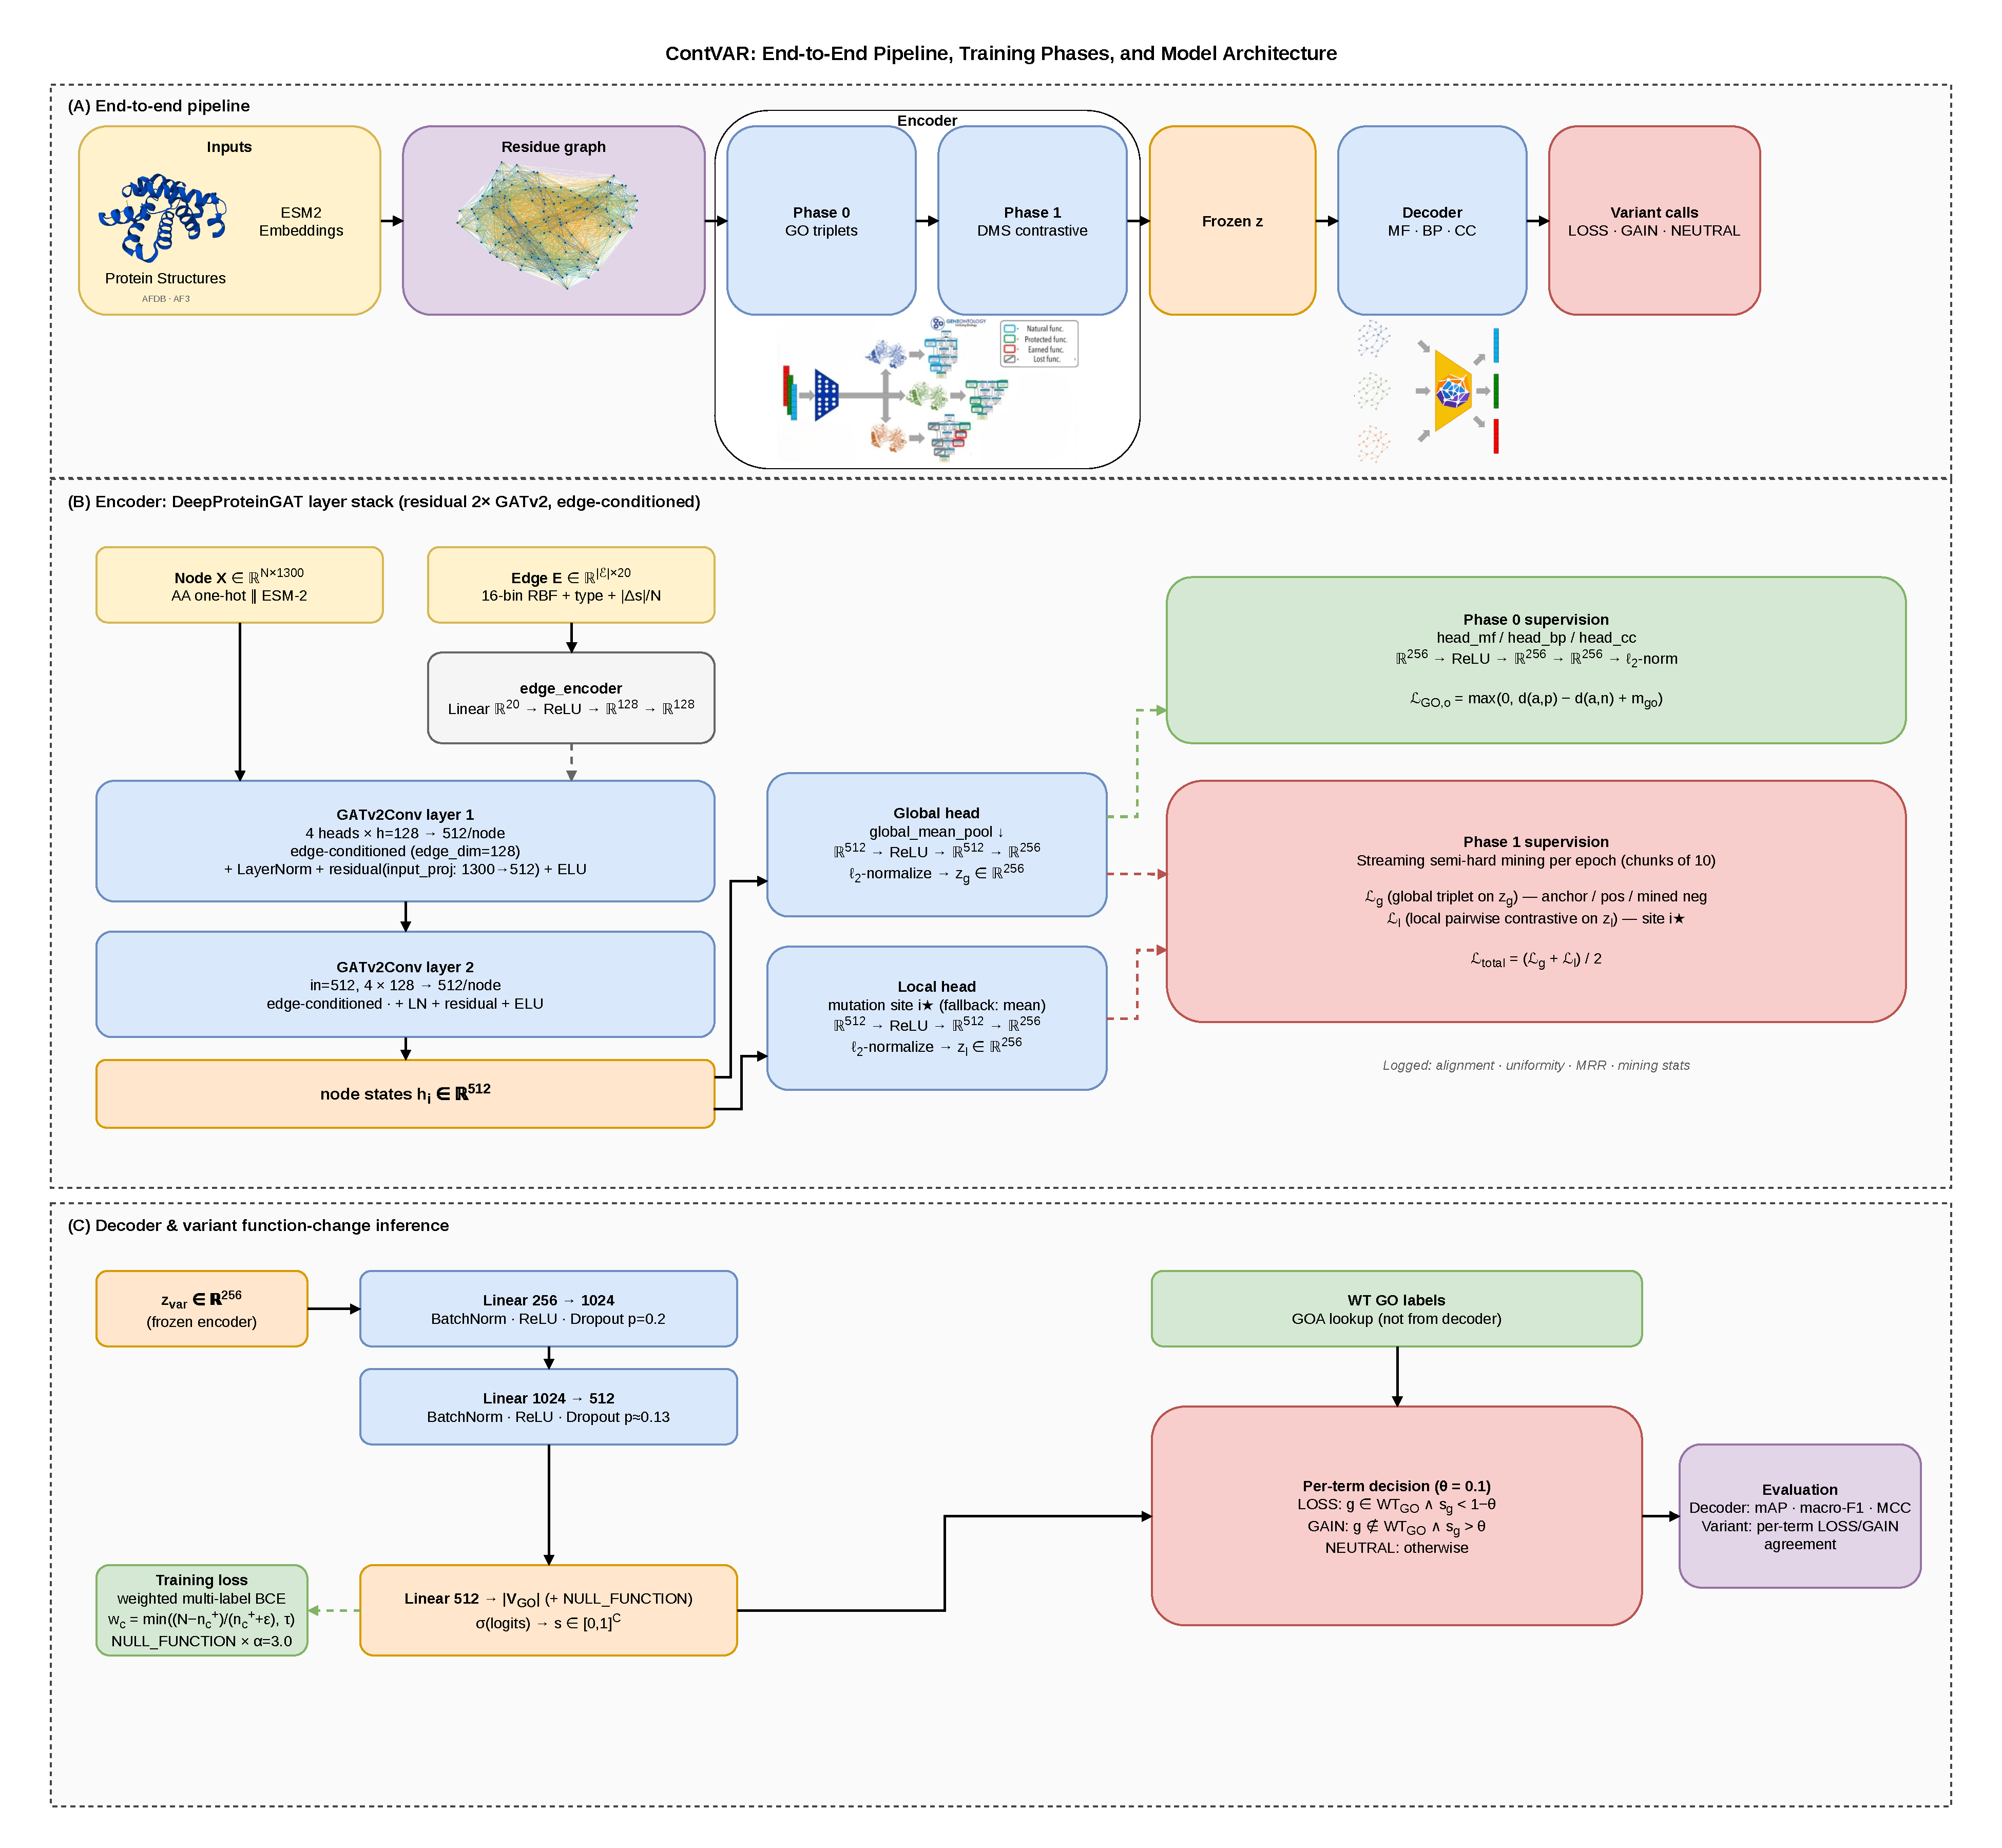
\includegraphics[width=\textwidth]{figures/contvar_pipeline_architecture.drawio.pdf}
  \vspace{-3pt}
  \caption{ContVAR end-to-end pipeline and model architecture.
  \textbf{(A)}~Data sources, hybrid residue-graph construction, and training stages: phase~0 GO semantic triplet pretraining, phase~1 DMS contrastive specialization with streaming semi-hard mining, and stage~2 per-aspect GO decoding with variant-level inference.
  \textbf{(B)}~Residual two-layer GATv2 encoder (\texttt{DeepProteinGAT}): edge-conditioned message passing, global mean-pooled and mutation-site local projection heads ($\mathbf{z}_g$, $\mathbf{z}_l \in \mathbb{R}^{256}$, $\ell_2$-normalized), and phase~1 joint $\mathcal{L}_g$--$\mathcal{L}_l$ objective.
  \textbf{(C)}~Per-ontology \texttt{FFNDecoder} and function-change calls (LOSS / GAIN / NEUTRAL, \texttt{ContVAR\_fitness}) from variant embeddings and wild-type GOA annotations.}
  \label{fig:pipeline}
\end{figure}

ContVAR is organized as two training stages that share a common protein identifier space:
\begin{enumerate}
    \item \textbf{Mutation-aware graph encoder.} Training proceeds in two phases. \textbf{Phase~0} performs GO semantic-similarity triplet pretraining with ontology-specific heads (MF, BP, CC) on residue graphs. \textbf{Phase~1} specializes the same backbone on DMS protein-family triplets with a joint global graph-level and local mutation-site contrastive loss; streaming semi-hard negative mining is active from the first phase~1 epoch.
    \item \textbf{Supervised GO decoder and variant function-change inference.} A feed-forward decoder (\texttt{FFNDecoder}) is trained on frozen encoder embeddings as a multi-label GO classifier under UniRef50 cluster-aware splits, separately for each GO aspect (MF, BP, CC). At inference, variant embeddings are scored and combined with curated wild-type (WT) GO annotations from GOA to produce per-GO LOSS / GAIN / NEUTRAL calls and a scalar \texttt{ContVAR\_fitness}.
\end{enumerate}
Encoder and decoder use different supervision signals---DMS-driven contrastive geometry versus protein-level GO multi-label annotations---and are linked through a persisted encoder checkpoint and protein embeddings keyed by UniProt identifier.

\subsection{Dataset Description}
\textbf{DMS (phase~1) track.} The mutagenesis corpus is organized by protein family with one wild-type anchor, multiple positives, and multiple negatives per family. Starting from the ProteinGym Deep Mutational Scanning benchmark~\cite{notin2023proteingym}, we retained proteins with sequence length at most 656 residues, giving 97 unique proteins. When an assay annotated only a protein segment, the corresponding full-length sequence was reconstructed and variant coordinates were remapped to the full-length residue index so that the graph encoder always received complete protein context. For each protein, the positive pool was built from 50 neutral variants selected immediately above the assay cutoff indicating retained-functionality while the negative pool used the 50 lowest-fitness score variants as deleterious examples; selection was sequence-position stratified to reduce clustering in a single domain or local region. This produced exactly 9,700 curated variants before graph construction. The DMS split respects the UniRef50-aware protein split used for phase~0 and decoder training: if a DMS protein is present in that split, the wild type and all of its variants inherit the same train/validation/test assignment; DMS proteins absent from the UniRef50 split are conservatively assigned to training. The resulting fixed DMS split contains 97 families (93 train, 2 validation, 2 test), preventing variant-level leakage across held-out protein families. Raw structures are consumed as mmCIF/CIF files, and per-residue ESM-2 embeddings are loaded from a precomputed store keyed by normalized protein identifiers. Mutated residue positions are parsed from variant filenames during collation and mining.

\textbf{GO (phase~0) track.} Phase~0 consumes residue graphs and ontology-specific semantic-similarity tables under the shared UniRef50-aware protein split, which contains 122,190 proteins (97,771 train, 12,093 validation, 12,326 test). Positives use similarity $\geq 0.8$; negatives use similarity $\leq 0.2$ and are sampled from low/mid bins ([0.0,0.1), [0.1,0.2]) for hardness balancing. 

\textbf{Structure interchange vs.\ cached graphs.} CIF/mmCIF is the portable format for atomic coordinates; serialized graph tensors cache parsing, featurization, and edge construction for reuse.

\subsection{Dataset Preparation / Preprocessing}
\textbf{From structures to residue graphs (DMS path).} Three-dimensional structures for the selected wild-type and variant sequences were generated with AlphaFold3. To reduce folding cost on the compute cluster, available assay/MSA resources were reused instead of regenerating alignments from scratch. The resulting mmCIF/CIF files are treated as fixed structural inputs for graph construction. Per-residue $\mathrm{C}_\alpha$ coordinates and amino-acid identities are extracted from these monomer structures and assembled into PyTorch Geometric graphs. Connectivity uses the hybrid edge scheme below; an optional pure $k$NN baseline (Graphein-style) is available for ablations.

Node features concatenate a residue-identity one-hot and a per-residue ESM-2 embedding:
\[
\mathbf{x}_i = [\text{AAOneHot}_i \, \| \, \text{ESM2}_i] \in \mathbb{R}^{20+1280} = \mathbb{R}^{1300}.
\]
ESM-2 (650M-parameter variant~\cite{lin2023evolutionary}) is chosen as the per-residue feature source because it produces high-quality sequence-contextualized representations without requiring multiple sequence alignment (MSA) construction at inference time. The embeddings are pre-computed and frozen throughout encoder training, so the GATv2 encoder learns mutation-sensitive spatial geometry on top of fixed evolutionary-chemical context rather than attempting to learn both from scratch.

\subsubsection{Hybrid residue-graph connectivity}
Deep mutational scanning (DMS) variants can alter both local side-chain packing and non-local residue coupling. A purely sequence-local chain graph under-represents 3D contacts; a fixed-radius spatial graph can miss compensatory long-range interactions; and a dense residue--residue graph is prohibitive for long chains. ContVAR therefore uses a \emph{fixed neighbor budget per residue} that mixes three complementary link types.

Let $N$ be the number of residues in a chain, $\mathbf{r}_i\in\mathbb{R}^3$ the $\mathrm{C}_\alpha$ coordinate of residue $i$, and $s_i$ its sequence index. Pairwise Euclidean distances $d_{ij}=\|\mathbf{r}_i-\mathbf{r}_j\|_2$ and index distances $|s_i-s_j|$ are computed within the same chain (cross-chain links are masked). For each residue $i$, neighbors are selected in three sequential stages; edges already chosen in an earlier stage are excluded from later stages:
\begin{enumerate}
    \item \textbf{Sequence-index neighbors} ($k_{\text{idx}}$, default 16): the $k_{\text{idx}}$ residues $j\neq i$ on the same chain with smallest $|s_i-s_j|$.
    \item \textbf{Spatial neighbors} ($k_{\text{sp}}$, default 16): among remaining candidates, the $k_{\text{sp}}$ residues with smallest $d_{ij}$.
    \item \textbf{Stochastic long-range neighbors} ($k_{\text{rnd}}$, default 16): among remaining candidates, sample $k_{\text{rnd}}$ partners via a Gumbel top-$k$ trick. Unnormalized scores are $w_{ij}=-3\log(d_{ij}+\epsilon)$; independent Gumbel noise is added and the lowest perturbed scores are taken, biasing selection toward closer residues while retaining diversity (inverse-cube weighting in distance space).
\end{enumerate}
Directed edges $(i\to j)$ are created for every valid neighbor slot; invalid padding slots ($j=-1$) are dropped. Each edge carries a 20-dimensional attribute vector: (i) a 16-bin Gaussian radial basis expansion of $d_{ij}$ on $[0,d_{\max}]$ with $d_{\max}=22$\,\AA; (ii) a 3-way one-hot encoding of neighbor type (index / spatial / random); and (iii) one normalized sequence separation $|s_i-s_j|/N$. The GATv2 stack consumes these attributes through an edge MLP before attention (Section~\ref{sec:encoder-backbone}).

This recipe is motivated by sparse-neighbor designs for structure modeling that combine chain-index, Euclidean nearest, and randomized long-range partners~\cite{jendrusch2025salad}; ContVAR adapts the connectivity pattern to residue-level message passing on AlphaFold-predicted monomers, with $k{=}16$ per neighbor type by default and on-disk graph caching when structures are revisited.

\textbf{Mutation context.} The encoder always sees the full-chain graph; locality around the variant is enforced in the loss via the mutation-site branch rather than by cropping the graph to a fixed-radius neighborhood.

\subsection{Model/Architecture Design}

\subsubsection{Mutation-Aware Graph Encoder (backbone)}
\label{sec:encoder-backbone}
The encoder is a residual two-layer GATv2 stack~\cite{brody2022how} with four attention heads per layer and hidden size 128. GATv2 is selected over standard GAT because the original GAT computes attention coefficients as a function of a linear combination of the concatenated source and target features, which Brody et al.~\cite{brody2022how} show collapses to a ranking over neighbors that is independent of the query node—making attention static. GATv2 remedies this by applying the non-linearity \emph{before} the attention projection so that each coefficient depends jointly on both the query and the key, yielding fully dynamic attention. In the context of irregular protein residue graphs, where the chemical environment around a mutation site varies substantially across different protein families and positions, this dynamic re-weighting is important: the encoder must learn to attend to non-local compensatory contacts whose relevance changes depending on which residue is mutated. Edge attributes are first projected by an MLP and injected into both GATv2 layers. Let $\mathbf{h}_i^{(l)}$ be node state at layer $l$; each layer applies attention-weighted aggregation with edge conditioning, layer normalization, and residual addition. Global embedding uses mean pooling followed by a projection head to 256 dimensions and $\ell_2$ normalization. A separate local projection head extracts the embedding at mutation position; if a residue index is absent, graph mean is used as fallback.

\subsubsection{Phase 0: GO semantic pretraining}
Phase~0 provides biologically informed initialization by training ontology-specific triplets (MF/BP/CC) using ontology heads on top of the shared encoder. For each ontology $o$:
\[
\mathcal{L}_{\text{GO},o}=\max(0,\ d(\mathbf{z}_a^o,\mathbf{z}_p^o)-d(\mathbf{z}_a^o,\mathbf{z}_n^o)+m_{go}),
\]
with default $m_{go}=0.2$. Active ontology losses are averaged per step. Optional ratio-based ontology sampling (default MF:BP:CC = 0.5:0.3:0.2) prevents dominance by a single ontology.

\subsubsection{Phase 1: DMS encoder training (global triplet + local contrastive loss)}
\label{sec:phase1-dms}
After phase~0, phase~1 loads DMS protein-family triplets under the UniRef50-respecting fixed split described above (97 families: 93 train, 2 validation, 2 test) and initializes weights from the phase~0 checkpoint. Phase~1 uses streaming semi-hard negative mining from the first training epoch: each epoch reshuffles protein families, samples positives, scans candidate negatives in chunks, and rebuilds mined batches online. Exhaustive positive$\times$negative enumeration is reserved for validation and test.

\paragraph{Per-batch mining and forward pass.}
Families are shuffled and grouped into mining batches of size 8. For each batch:
\begin{enumerate}
    \item One positive variant per family is sampled; anchor and positive residue graphs are loaded from cache or built on the fly.
    \item The current model embeds anchors and positives (no gradient) to obtain $d_{ap}=d(\mathbf{z}_a^g,\mathbf{z}_p^g)$.
    \item All candidate negatives listed for that family are scanned in chunks of 10 structures; negatives that are hard ($d_{an}<d_{ap}$) or semi-hard ($d_{ap}\le d_{an}<d_{ap}+m$) are retained and up to 10 per family are subsampled at random; if none qualify, the closest negative is used.
    \item A gradient step runs on the mined set; the global triplet hinge $\max(0, d_{ap}-d_{an}+m)$ is averaged over all qualifying negatives in the batch.
\end{enumerate}
The global loss is therefore always computed on mined hard/semi-hard negatives, not on a fixed random subset chosen once per epoch.

\paragraph{Losses.}
For mined negatives, the global branch is
\[
\mathcal{L}_{g}=\frac{1}{|\mathcal{Q}|}\sum_{n\in\mathcal{Q}}\max\bigl(0,\ d(\mathbf{z}_a^g,\mathbf{z}_p^g)-d(\mathbf{z}_a^g,\mathbf{z}_n^g)+m\bigr),
\]
where $\mathcal{Q}$ is the set of hard and semi-hard negatives retained for the batch. The local branch supervises mutation-site embeddings. Global mean pooling can dilute mutation-specific signal in long proteins; the local head extracts the embedding at the parsed mutation index and applies a pairwise contrastive loss that attracts anchor--positive pairs and repels anchor--negative pairs at the mutation site:
\[
\mathcal{L}_{l}=\frac{1}{2B}\sum_{i=1}^{2B}\left[y_i d_i^2 + (1-y_i)\max(0,m-d_i)^2\right],
\]
with $y_i=1$ on positive pairs and $y_i=0$ on negative pairs. The hardest global negative per family (index from mining stats) is reused to select which mutation-site negative enters $\mathcal{L}_l$. The step objective is
\[
\mathcal{L}_{\text{total}}=\frac{\mathcal{L}_{g}+\mathcal{L}_{l}}{2}.
\]

\paragraph{Optimization, validation, and checkpoints.}
Phase~1 training runs for 200 epochs by default. Optimizer: AdamW (learning rate $10^{-4}$, weight decay 0.01) with gradient accumulation over four steps and gradient clipping at norm 1.0. Validation and test enumerate every positive$\times$negative pair per family for stable ranking metrics. The phase~1 checkpoint with lowest validation $\mathcal{L}_{\text{total}}$ is retained for embedding export and decoder training.

\subsubsection{Supervised GO decoder}
\label{sec:decoder}

\paragraph{Scope.}
The decoder consumes protein-level embeddings from the trained encoder (256 dimensions) or, in ablations, raw ESM-2 embeddings (1{,}280 dimensions). It outputs multi-label GO probabilities under Molecular Function (MF), Biological Process (BP), and Cellular Component (CC). One decoder is trained independently per aspect.

\paragraph{GO annotation source and vocabulary.}
Labels are taken from UniProt-GOA Swiss-Prot, excluding electronic (\texttt{IEA}) and ``no data'' (\texttt{ND}) evidence codes. The vocabulary retains GO terms annotated in at least ten training proteins. A dedicated \texttt{NULL\_FUNCTION} class is appended to flag predicted complete loss of function.

\paragraph{Dataset and UniRef50-aware splits.}
Training proteins are partitioned by UniRef50 cluster so that no cluster appears in more than one of train, validation, or test. This same protein-level partition is used by phase~0 and by all three decoder aspects, and the DMS family split inherits it where the DMS protein is present in the UniRef50 mapping. Each protein is represented by a multi-hot label vector over the aspect vocabulary.

\paragraph{Architecture.}
\texttt{FFNDecoder} is a feed-forward network with hidden widths $512 \to 1024 \to 512$, batch normalization, ReLU activations, and dropout ($p=0.3$, tapered in the last hidden block). The head outputs logits per GO term; sigmoid is applied at inference.

\paragraph{Class-balanced multi-label loss.}
Training uses binary cross-entropy with logits and positive-class weights. For GO term $c$,
\[
w_c \;=\; \min\!\left(\frac{N - n_c^{+}}{n_c^{+}+\varepsilon},\ \tau\right),\qquad
w_{\text{NULL\_FUNCTION}} \;\leftarrow\; \alpha \cdot w_{\text{NULL\_FUNCTION}},
\]
where $n_c^{+}$ is the number of training proteins with term $c$, $N$ is the training set size, $\tau=20$, and $\alpha=3.0$.

\paragraph{Optimization and schedule.}
AdamW with learning rate $10^{-3}$ and weight decay $10^{-4}$; cosine annealing over 100 epochs; batch size 256. The best validation mAP checkpoint is kept; training stops if mAP fails to improve by more than $10^{-4}$ for ten consecutive epochs. Metrics are logged to Weights \& Biases.

\paragraph{Decoder evaluation metrics.}
Validation and test use logits converted to probabilities. GO terms with zero positives in a split are excluded from mAP. At probability threshold 0.95 we report macro-averaged F1, precision, recall, subset accuracy, and MCC.

\paragraph{Variant function-change inference.}
The decoder is run on \emph{variant} embeddings only; wild-type GO annotations are looked up directly from GOA (the database is the source of truth for the WT). For a variant with embedding $\mathbf{z}_{\text{var}}$ let $\mathbf{s}=\sigma(\text{FFNDecoder}(\mathbf{z}_{\text{var}}))\in[0,1]^C$. For each annotated WT GO term $g$:
\[
\text{status}(g) =
\begin{cases}
\text{LOSS} & \text{if } g \in \mathrm{WT}_{\text{GO}} \text{ and } s_g < 1-\theta,\\
\text{GAIN} & \text{if } g \notin \mathrm{WT}_{\text{GO}} \text{ and } s_g > \theta,\\
\text{NEUTRAL} & \text{otherwise,}
\end{cases}
\]
with default $\theta=0.1$. A single scalar
\[
\mathrm{ContVAR\_fitness} \;=\; \frac{1}{|\mathrm{WT}_{\text{GO}}|}\sum_{g\in \mathrm{WT}_{\text{GO}}} s_g
\]
is computed over the GO terms annotated in the wild type (excluding \texttt{NULL\_FUNCTION}). $\mathrm{ContVAR\_fitness}\!\approx\!1.0$ means the variant is predicted to retain all WT functions, while values approaching $0.0$ correspond to broad function loss.

\paragraph{Batch variant scoring.}
Variant embeddings are scored in batch; wild-type accessions and mutation tokens are parsed from record identifiers. Variants whose wild type lacks GOA coverage are skipped. When experimental binary labels are available, AUROC and AUPRC of \texttt{ContVAR\_fitness} against the label summarize variant-level agreement with assays.

\subsection{Evaluation Metrics}

\paragraph{Encoder-side metrics.}
During phase~0 and phase~1 we log total, global, and local losses; mean reciprocal rank (MRR), alignment, and uniformity on $\ell_2$-normalized embeddings; global and local distance margins; and per-batch counts of hard, semi-hard, and easy mined negatives. Validation and test use exhaustive positive$\times$negative combinations per family. The encoder checkpoint with lowest validation total loss is re-evaluated on held-out families before decoder training.

\paragraph{Decoder-side metrics.}
Each aspect (MF, BP, CC) is evaluated under the shared UniRef50 cluster-aware split. We report mAP over terms with at least one positive in the split, and at threshold 0.95 macro-averaged F1, precision, recall, accuracy, and MCC. The validation mAP-best model is evaluated on the test split.

\paragraph{Variant-level metrics.}
When experimental variant labels are available (e.g.\ ProteinGym-style fitness), we report AUROC and AUPRC of \texttt{ContVAR\_fitness}, mean fitness per label class, and counts of LOSS / GAIN / NEUTRAL calls per variant.

\section{Results and Discussion}

Results below are reported as placeholders until final training runs are consolidated; table layouts are fixed so that partial numbers from W\&B or internal logs can be dropped in without restructuring. Decoder comparisons use three \emph{embedding sources} for the same \texttt{FFNDecoder} architecture and training recipe (UniRef50 cluster-aware splits, threshold 0.95 for thresholded metrics):
\begin{itemize}
    \item \textbf{ContVAR (full):} encoder after phase~0 and phase~1 (256-d graph embeddings).
    \item \textbf{ESM-2 baseline:} raw 650M ESM-2 protein embeddings (1{,}280-d), no ContVAR encoder.
    \item \textbf{Phase-0 encoder:} embeddings from the GO-pretrained encoder only, without phase~1 DMS fine-tuning (256-d).
\end{itemize}

\subsection{Encoder: phase~1 (DMS) metrics}
Phase~1 contrastive training is evaluated on the held-out DMS families with exhaustive anchor--positive--negative pairs. Table~\ref{tab:encoder-main} reports the \textbf{ContVAR (full)} encoder at its best validation checkpoint; phase-0-only and random-init encoder ablations can be added alongside if needed.

\begin{table}[h]
\centering
\caption{Encoder metrics on the DMS family split at the best phase~1 validation checkpoint (\textbf{ContVAR full} encoder: phase~0 + phase~1).}
\label{tab:encoder-main}
\begin{tabular}{lcc}
\hline
Metric & Validation & Test \\
\hline
Loss (total) & [\_] & [\_] \\
Loss (global) & [\_] & [\_] \\
Loss (local) & [\_] & [\_] \\
MRR & [\_] & [\_] \\
Alignment & [\_] & [\_] \\
Uniformity & [\_] & [\_] \\
\hline
\end{tabular}
\end{table}

\subsection{Decoder: wild-type GO function prediction (validation and test)}
Wild-type proteins are scored with one decoder per GO aspect (MF, BP, CC). Table~\ref{tab:decoder-ablation} compares the three embedding sources on the standard UniRef50-based annotation val/test split (protein-level multi-label GO prediction).

\begin{table}[h]
\centering
\small
\caption{Decoder ablation on wild-type GO annotation. Rows group by embedding source and aspect; Val/Test are the held-out protein splits. mAP excludes terms with zero positives in that split; F1, precision, recall, accuracy, and MCC are macro-averaged at probability threshold 0.95.}
\label{tab:decoder-ablation}
\begin{tabular}{lllcccccc}
\hline
Embedding source & Aspect & Split & mAP & F1$_{\text{macro}}$ & Prec. & Rec. & Acc. & MCC \\
\hline
ContVAR (full) & MF & Val  & [\_] & [\_] & [\_] & [\_] & [\_] & [\_] \\
ContVAR (full) & MF & Test & [\_] & [\_] & [\_] & [\_] & [\_] & [\_] \\
ContVAR (full) & BP & Val  & [\_] & [\_] & [\_] & [\_] & [\_] & [\_] \\
ContVAR (full) & BP & Test & [\_] & [\_] & [\_] & [\_] & [\_] & [\_] \\
ContVAR (full) & CC & Val  & [\_] & [\_] & [\_] & [\_] & [\_] & [\_] \\
ContVAR (full) & CC & Test & [\_] & [\_] & [\_] & [\_] & [\_] & [\_] \\
\hline
ESM-2 baseline & MF & Val  & [\_] & [\_] & [\_] & [\_] & [\_] & [\_] \\
ESM-2 baseline & MF & Test & [\_] & [\_] & [\_] & [\_] & [\_] & [\_] \\
ESM-2 baseline & BP & Val  & [\_] & [\_] & [\_] & [\_] & [\_] & [\_] \\
ESM-2 baseline & BP & Test & [\_] & [\_] & [\_] & [\_] & [\_] & [\_] \\
ESM-2 baseline & CC & Val  & [\_] & [\_] & [\_] & [\_] & [\_] & [\_] \\
ESM-2 baseline & CC & Test & [\_] & [\_] & [\_] & [\_] & [\_] & [\_] \\
\hline
Phase-0 encoder & MF & Val  & [\_] & [\_] & [\_] & [\_] & [\_] & [\_] \\
Phase-0 encoder & MF & Test & [\_] & [\_] & [\_] & [\_] & [\_] & [\_] \\
Phase-0 encoder & BP & Val  & [\_] & [\_] & [\_] & [\_] & [\_] & [\_] \\
Phase-0 encoder & BP & Test & [\_] & [\_] & [\_] & [\_] & [\_] & [\_] \\
Phase-0 encoder & CC & Val  & [\_] & [\_] & [\_] & [\_] & [\_] & [\_] \\
Phase-0 encoder & CC & Test & [\_] & [\_] & [\_] & [\_] & [\_] & [\_] \\
\hline
\end{tabular}
\end{table}

\subsection{Variant-level evaluation on DMS assay labels}
For variants with experimental fitness or pathogenicity labels in the DMS corpus, \texttt{ContVAR\_fitness} from the \textbf{ContVAR (full)} pipeline is correlated with the binary assay label (Table~\ref{tab:variant-dms}). The same three embedding/decoding conditions as Table~\ref{tab:decoder-ablation} can be reported here if variant scoring is repeated per model.

\begin{table}[h]
\centering
\caption{Variant-level metrics on the DMS-labeled variant pool (\texttt{ContVAR\_fitness} vs.\ experimental label). Primary row block: ContVAR (full); add ESM-2 baseline and phase-0 encoder rows when variant embeddings are exported for those conditions.}
\label{tab:variant-dms}
\begin{tabular}{llcccccc}
\hline
Embedding source & Aspect & AUROC & AUPRC & $\overline{\text{fit}}_{y=0}$ & $\overline{\text{fit}}_{y=1}$ & $n_{\text{pred}}$ & $n_{\text{skip}}$ \\
\hline
ContVAR (full) & MF & [\_] & [\_] & [\_] & [\_] & [\_] & [\_] \\
ContVAR (full) & BP & [\_] & [\_] & [\_] & [\_] & [\_] & [\_] \\
ContVAR (full) & CC & [\_] & [\_] & [\_] & [\_] & [\_] & [\_] \\
ESM-2 baseline & MF & [\_] & [\_] & [\_] & [\_] & [\_] & [\_] \\
ESM-2 baseline & BP & [\_] & [\_] & [\_] & [\_] & [\_] & [\_] \\
ESM-2 baseline & CC & [\_] & [\_] & [\_] & [\_] & [\_] & [\_] \\
Phase-0 encoder & MF & [\_] & [\_] & [\_] & [\_] & [\_] & [\_] \\
Phase-0 encoder & BP & [\_] & [\_] & [\_] & [\_] & [\_] & [\_] \\
Phase-0 encoder & CC & [\_] & [\_] & [\_] & [\_] & [\_] & [\_] \\
\hline
\end{tabular}
\end{table}

\subsection{Variant function-change cohort}
Separately from the DMS assay pool, we evaluate variants in a curated \textbf{function-change cohort}: proteins with experimentally supported or manually verified GO-level loss or gain of function upon mutation (cohort assembly in progress). This set stresses whether LOSS/GAIN/NEUTRAL calls and \texttt{ContVAR\_fitness} align with known function-change cases rather than bulk fitness ranking alone. Table~\ref{tab:variant-funcchange} will report the same embedding-source comparison; numbers to be filled from the cohort evaluation pipeline.

\begin{table}[h]
\centering
\caption{Performance on the variant \textbf{function-change cohort} (curated proteins with annotated GO function change). Metrics mirror Table~\ref{tab:variant-dms} but restricted to cohort members; optional columns for per-class LOSS/GAIN/NEUTRAL agreement can be added when labels are finalized.}
\label{tab:variant-funcchange}
\begin{tabular}{llcccccc}
\hline
Embedding source & Aspect & AUROC & AUPRC & $\overline{\text{fit}}_{y=0}$ & $\overline{\text{fit}}_{y=1}$ & $n_{\text{cohort}}$ & $n_{\text{skip}}$ \\
\hline
ContVAR (full) & MF & [\_] & [\_] & [\_] & [\_] & [\_] & [\_] \\
ContVAR (full) & BP & [\_] & [\_] & [\_] & [\_] & [\_] & [\_] \\
ContVAR (full) & CC & [\_] & [\_] & [\_] & [\_] & [\_] & [\_] \\
ESM-2 baseline & MF & [\_] & [\_] & [\_] & [\_] & [\_] & [\_] \\
ESM-2 baseline & BP & [\_] & [\_] & [\_] & [\_] & [\_] & [\_] \\
ESM-2 baseline & CC & [\_] & [\_] & [\_] & [\_] & [\_] & [\_] \\
Phase-0 encoder & MF & [\_] & [\_] & [\_] & [\_] & [\_] & [\_] \\
Phase-0 encoder & BP & [\_] & [\_] & [\_] & [\_] & [\_] & [\_] \\
Phase-0 encoder & CC & [\_] & [\_] & [\_] & [\_] & [\_] & [\_] \\
\hline
\end{tabular}
\end{table}

\subsection{Additional ablations and analyses}
\textit{[Placeholder.]} Beyond Table~\ref{tab:decoder-ablation}, planned encoder-side ablations include hybrid vs.\ $k$NN edges, GO-pretrained vs.\ random-init encoder before phase~1, global-only vs.\ local-only vs.\ joint $\mathcal{L}_g+\mathcal{L}_l$, and mining strategy. Decoder-side threshold sweeps around 0.95 and \texttt{NULL\_FUNCTION} loss weighting remain optional sensitivity analyses.

\subsection{Qualitative or case studies}
\textit{[Placeholder.]} Suggested case-study outputs available in project tooling:
\begin{itemize}
\item t-SNE projection of anchor/positive/negative embeddings on held-out families.
\item Hard-negative inspection: examples with smallest global anchor--negative distances under streaming mining.
\item Mutation-site local-distance profiles for selected variants.
\item Per-variant LOSS/GAIN/NEUTRAL summaries for well-studied disease variants with WT GO from GOA.
\end{itemize}

\section{Conclusion and Future Work}

\subsection{Conclusion}
Accurate, mechanistically informative variant interpretation requires models that respect both molecular structure and large-scale functional assays, and that translate the resulting representations back into the ontology-level vocabulary that biologists actually use. ContVAR addresses both halves of this requirement with a two-stage pipeline: (i) a residual GATv2 encoder over ESM-augmented residue graphs, trained with GO semantic-similarity triplet pretraining (phase~0) across MF/BP/CC followed by phase~1 DMS specialization with a joint global triplet plus mutation-local contrastive loss under streaming semi-hard mining; and (ii) three per-aspect feed-forward decoders, trained with class-balanced multi-label BCE (including a dedicated \texttt{NULL\_FUNCTION} class) under a UniRef50 cluster-aware split, that turn variant embeddings into per-GO LOSS / GAIN / NEUTRAL calls and a scalar \texttt{ContVAR\_fitness}.

\subsection{Future Work}
\textit{[Placeholder.]}

\bibliographystyle{IEEEtran}
\bibliography{reference}

\end{document}
